\chapter{Security of Connect IQ store}
\section{Preliminary analysis}
\begin{figure}[h]
    \centering
    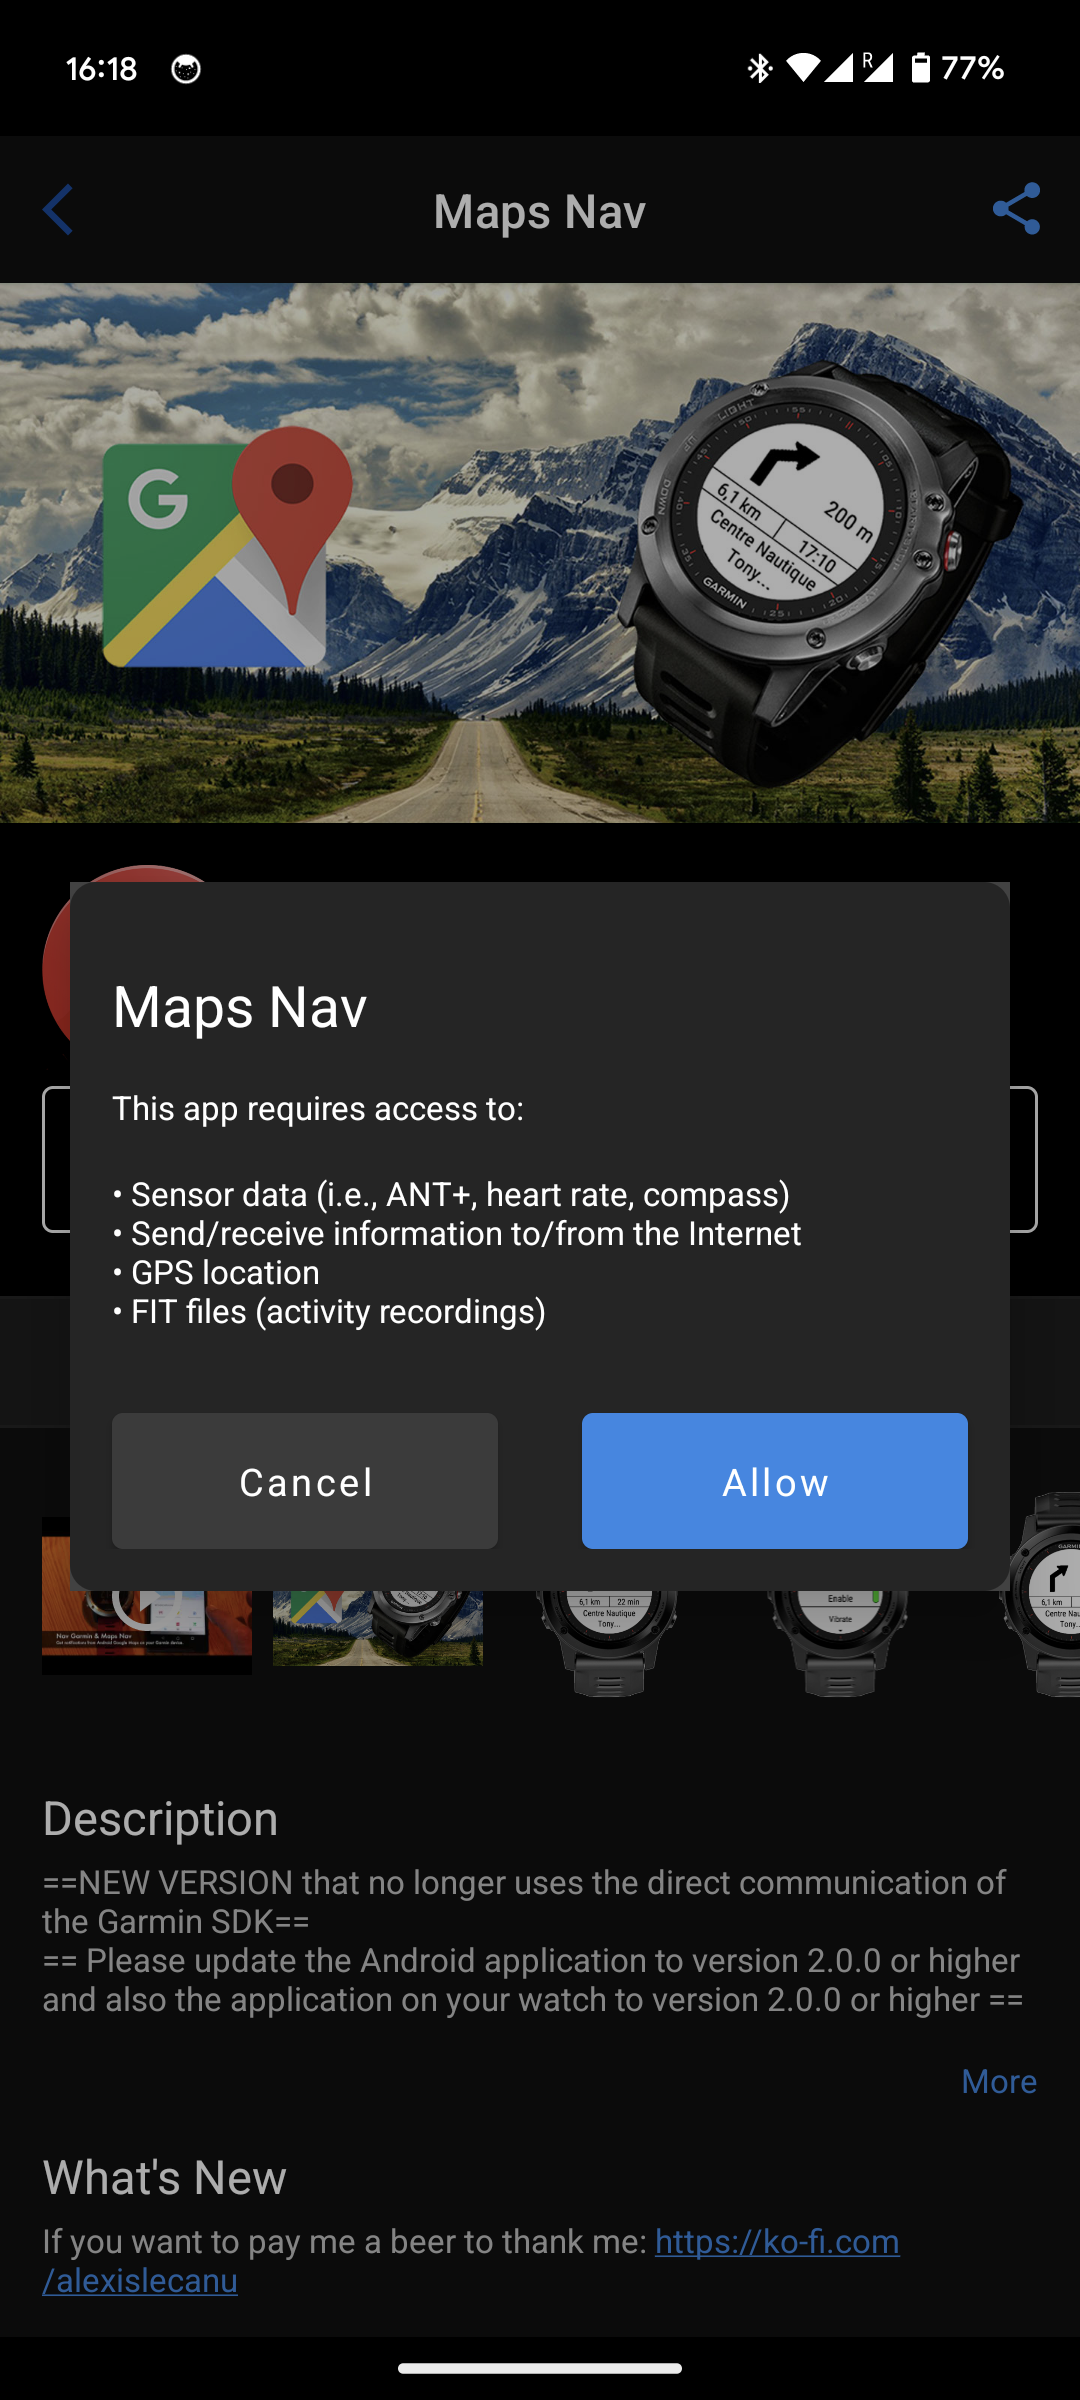
\includegraphics[width=0.3\linewidth]{../../images/connect-iq-app-permissions}
    \caption{Connect IQ - third-party app permissions request}
    \label{fig:connect-iq-store-permissions}
\end{figure}
Connect IQ store allows the users to browse and download third-party apps and watch faces to the watch.
The applications have descriptions and screenshots that can be added by the developers.
Additionally, users can write reviews and rate the apps.
Each app has information about the average rating and the number of downloads.
Before the app is downloaded, the user is presented with the information about permissions that the app requires, as presented in Figure~\ref{fig:connect-iq-store-permissions}.
The store also allows the users to create their own simple watch faces.

Based on the experiments with the watch, it seems that the app is downloaded to the phone and then sent to the watch via Bluetooth.

The analysis of the store does not go very deep, as I decided to focus more on the third-party apps.
However, it was necessary to have a basic understanding of the store, especially to analyze the communication between the watch and the phone.
This is described in the section~\ref{subsec:communication-watch-phone}.

\section{App decompilation}
\begin{figure}[h]
    \centering
    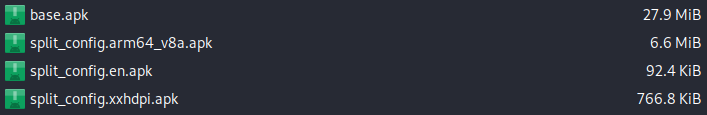
\includegraphics[width=0.7\linewidth]{../../images/connect-iq-apks}
    \caption{Connect IQ - Pulled apk files}
    \label{fig:connect-iq-apks}
\end{figure}
I installed the app on the phone and used $ADB$ to pull the apk files, that are presented in Figure~\ref{fig:connect-iq-apks}.
The app consists of multiple files, but the main one is \texttt{base.apk}.
It contains all JVM bytecode, which is the main focus of the analysis.
I decompiled the app with the JADX decompiler\footnote{\url{https://github.com/skylot/jadx}}.

The app is obfuscated.
It is a good practice as it makes the app size smaller and makes it more difficult to reverse engineer.
I was interested to find the code responsible for downloading the app to the phone and sending it to the watch.
Searching with several keywords, I was not able to find any code that would be responsible for checking the certificate of the downloaded app.
I was looking for names such as the library that was used to sign the app, SHA1, RSA\@.

Assuming that the watch is checking the certificate, it is not necessary for the phone to check it as well.
This is way it should be even safer, as the phone would be an additional attack surface.
With this conclusion, I decided to experiment later with the installation of an app that was not signed by the store in section~\ref{app-sideloading}.
%\section{Static analysis}
%
%Domain config is insecurely configured to permit clear text traffic to these domains in scope.
%
%It was detected that the is signed with MD5.
%MD5 hash algorithm is known to have collision issues.
%I couldnt verify it, to my knowledge the app was signed correctly.
%With signing scheme v2 and v3



\section{Sniffing the traffic}
To analyze the network security, I tried to sniff the traffic between the phone and Garmin servers.
I decided to use mitmproxy\footnote{\url{https://mitmproxy.org/}}.
When performing a dynamic analysis, there are two options.
Either use an emulator or a real device.
Emulator usually offers more flexibility and is easier to manipulate.
However, it does not have access to Bluetooth, which is necessary to test the Connect IQ store.
For this reason, I used a real device.

\begin{figure}[h]
    \centering
    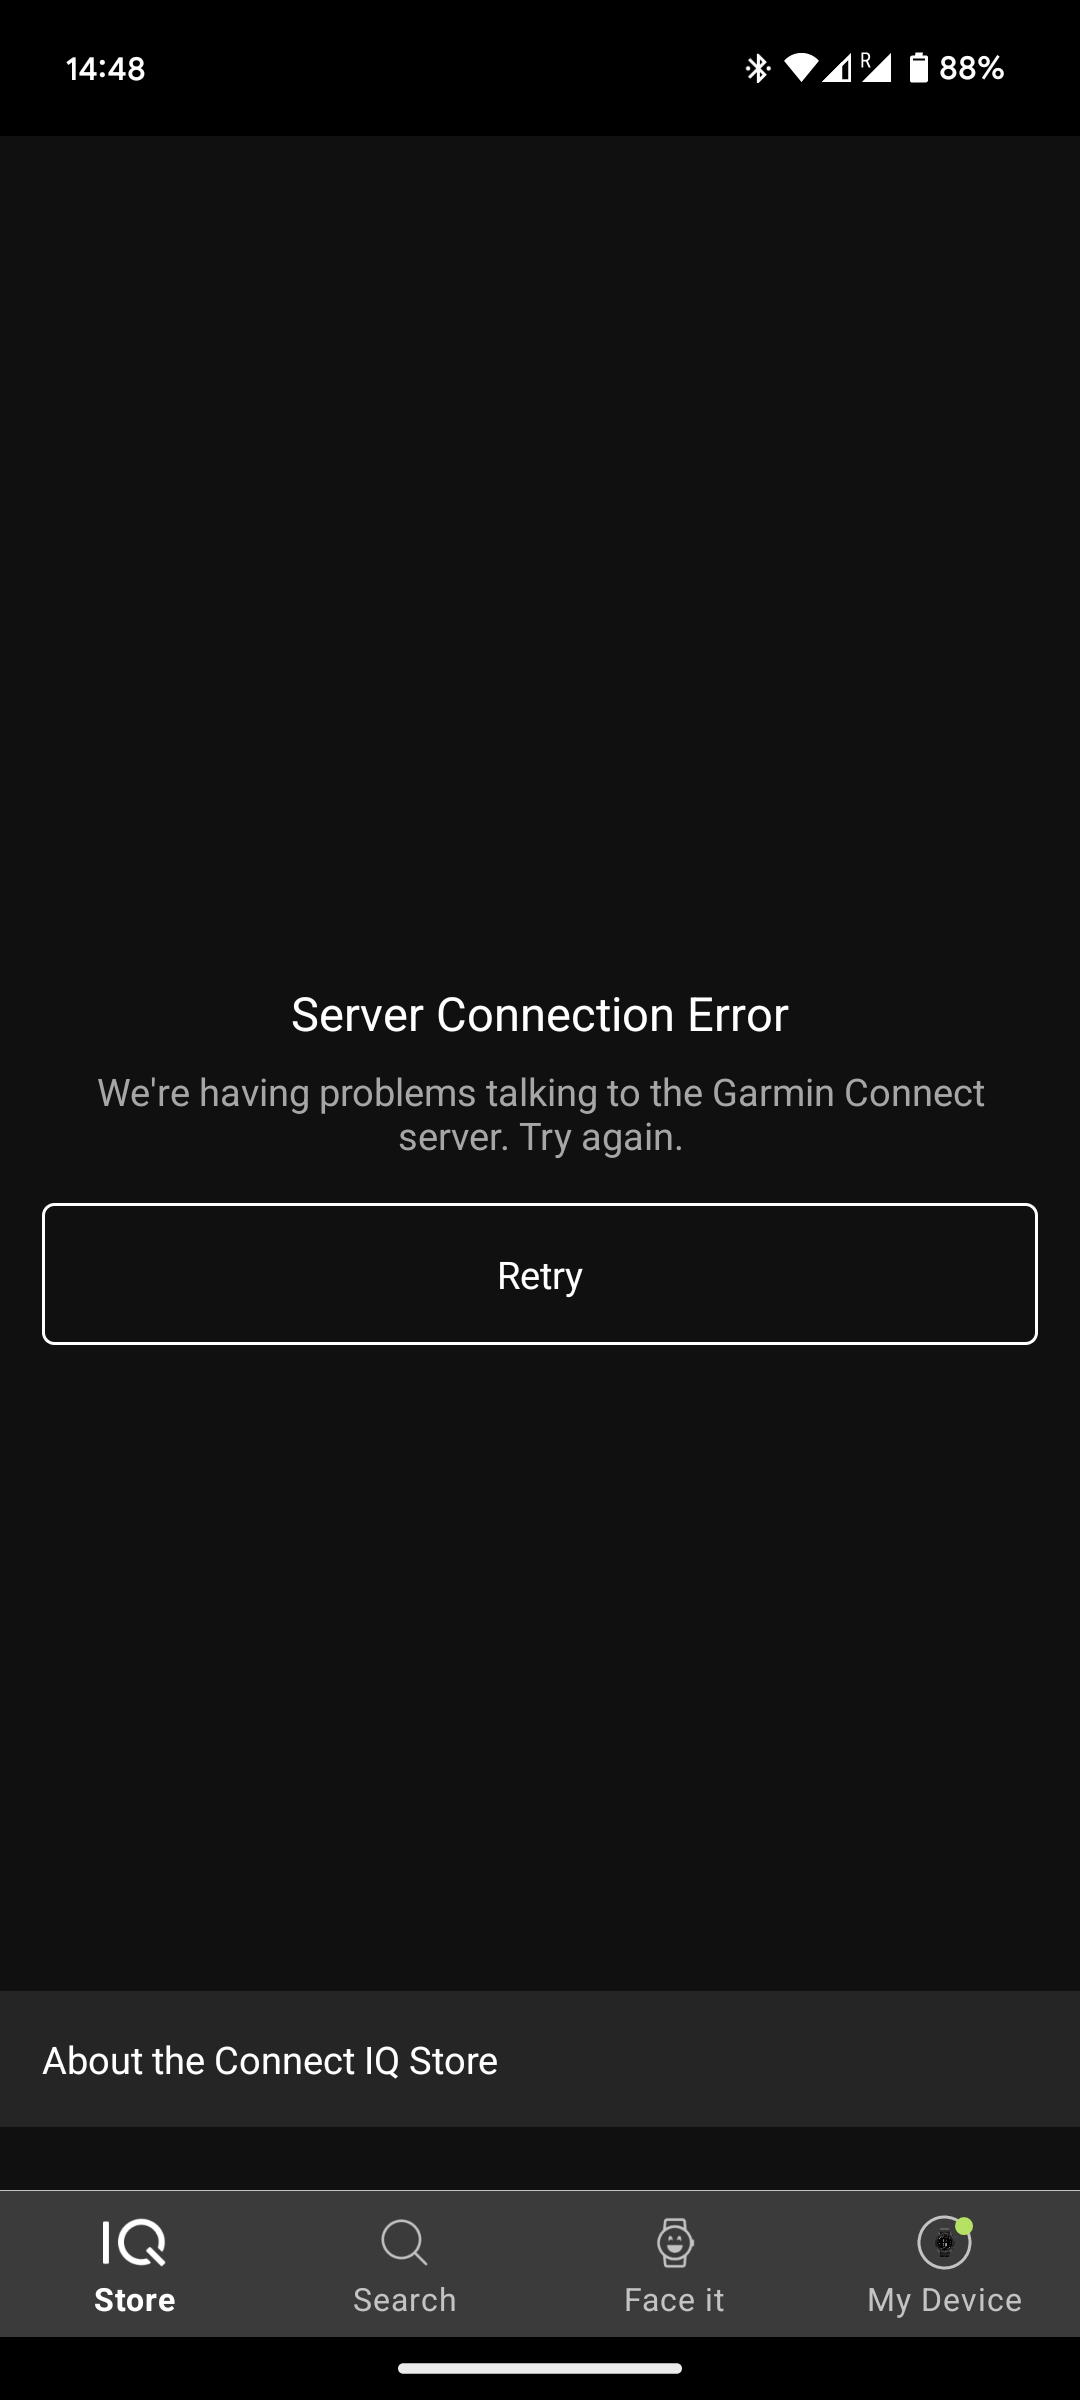
\includegraphics[width=0.3\linewidth]{../../images/connect-iq-connection-failed}
    \caption{Connect IQ refusing to connect}
    \label{fig:connect-iq-connection-failed}
\end{figure}

I configured the computer to act as a hotspot, started mitmproxy and forwarded the traffic there.
Then I connected the phone to the hotspot, and I was able to capture the traffic.
However, when connecting to the mitmproxy, the app refused to connect, as presented in Figure~\ref{fig:connect-iq-connection-failed}.
This means that the app is checking the certificate of the server and man-in-the-middle attack is not easy to execute.
After adding the mitmproxy certificate to the phone, the app would still refuse to connect.
The app is probably using a default Android certificate configuration, which does not trust user added certificates.
This is the case for all recent Android versions.
As the minimum supported version by Connect IQ is Android 7, it would be required to have root access to add certificates accepted by applications.
Another option is to modify the app to accept user added certificates.

\subsection*{Attempt 1 — Android Unpinner}
I tried to use Android Unpinner\footnote{\url{https://github.com/mitmproxy/android-unpinner}}.
It is an open-source tool that modifies the app to remove certificate pinning.
After installing the modified app, it was possible to sniff the traffic.
However, it was not possible to log in.
When trying to do so, it would go back to the welcome screen every time.

\subsection*{Attempt 2 — manually modify the apk and sign again}

I decided to try to modify the app manually.
I used Apktool\footnote{\url{https://apktool.org/}} to unpack the app.
Then I modified the network security configuration file to accept the user added certificates.
After that, I packed it again, aligned zip file and signed with a debug key.
After installing the app, there were some errors with missing resources.
I did not investigate it further.

\subsection*{Attempt 3 — only resign the app.}

To check if there is any potential in this approach, I decided to try to resign the app without any modifications and any proxy.
The app started, but again it was not possible to log in, it would go back to the welcome screen as in the first attempt.
I was not able to find what was the reason for that.
I could not find anything in the request logs from mitmproxy.
Sometimes hash of the fingerprint is used to identify the app by some services.
However, I did not find any evidence of that.

\subsection*{Attempt 4 — use rooted phone}
After the previous failed attempts, I decided to try to use a rooted phone.
I used my old, no longer used phone — Samsung S20.
To root the phone, I followed the instructions found on the XDA Forums\footnote{\url{https://xdaforums.com/t/how-to-exynos-snapdragon-root-s20-series-and-upgrade-firmware.4079353/}}.
Then I was able to install the mitmproxy certificate as the system certificate and use the original app.

\section{Network security}
Finally, I was able to sniff the traffic, as presented in Figure~\ref{fig:mitmproxy-unpinner}.
Based on the traffic that went through mitmproxy, I was able to determine Garmin domains used by the app.
I used Qualys SSl Labs\footnote{\url{https://www.ssllabs.com/ssltest/}} to analyze their security.

\begin{itemize}
    \item \textit{sso.garmin.com} - Received grade B because the server still supports TLS 1.1.
    It is not optimal, as there are known vulnerabilities of this protocol.
    \item \textit{diauth.garmin.com} - Received grade A, analysis did not find any issues.
\end{itemize}

\begin{figure}[h]
    \centering
    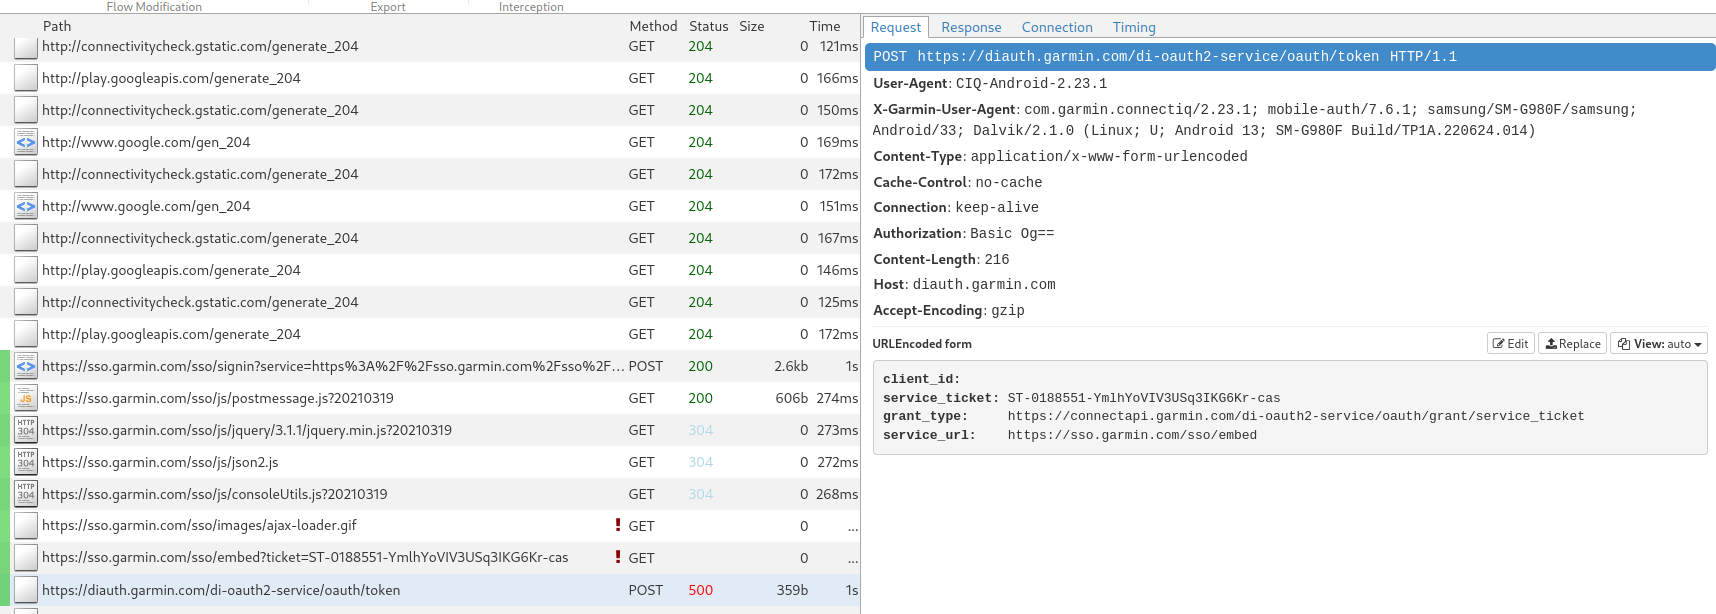
\includegraphics[width=1\linewidth]{../../images/mitmproxy unpinner}
    \caption{Sniffed traffic}
    \label{fig:mitmproxy-unpinner}
\end{figure}

Additionally, as the app allows the users to add their content, I looked at how it is handled.
The developer creates a description of their app, screenshots, and other information.
Moreover, other users can comment on the app.
With this type of content, it is important to be aware of potential attacks if the text is not parsed correctly.
Fortunately, in the case of native Android apps, usually attacks known from web applications are not possible.
Nonetheless, if the text is not parsed correctly, it could be a potential vector of attack.
However, it seems that everything is sent as a plain text.
It looks like there are no tags or any special parsing.
In this case, it should not be possible to perform any attacks based on improper sanitization of the input.
%\section{Communication between the watch and the phone}
%I considered analyzing the communication between the watch and the phone.
%However, it uses Bluetooth LE Secure Connections.

\section{App sideloading}
\label{app-sideloading}
Garmin allows the developers to install the app on the watch through the cable.
I was interested to see if it is possible to install an app not signed by the store remotely.
I tested it by replacing the app that would be downloaded from the store with the one that I created.
When the app is installed, the phone downloads the app from the store and sends it to the watch.
With the help of the mitmproxy, I was able to capture the request and replace the app with a different one.
After experimenting with different apps, the watch would refuse to install any app not signed by the store.
It was possible, however, to replace the app with another one, signed by the store.
This means that the watch is probably checking the certificate of the app.

It suggests that the API for remote app installation requires the app to be signed by the store.
This is a good thing, as it helps to prevent the installation of malicious apps.
